% !TeX program = pdflatex
\documentclass[11pt,twoside,a4paper]{article}
\usepackage{styleAND_2023}
\usepackage{xurl}% переносимые DOI в списке литературы
\captionsetup[table]{labelsep=period}
% Подзаголовки на отдельной строке (не в подбор)
\makeatletter
\renewcommand{\subsection}{\@startsection{subsection}%
  {1}{0pt}{0.25cm}{0.4cm}%
  {\bfseries\raggedright}%
}
\makeatother% отделяем номер таблицы от заголовка
\emergencystretch=2em% устранение редких переполнений строк

%%%%%%%%%%%%%%%%%%%%%%%%%%%%%%%%%%%%%%%%%%%%%%%%%%%%%%%%%%%%%%%%%%%%%%%%%%%%%%%
%%% ПОЛЯ, КОТОРЫЕ ДОЛЖЕН ЗАПОЛНИТЬ АВТОР ПЕРЕД ПОДАЧЕЙ (метка ЗАПОЛНИТЬ): %%%
%%% 1. \authors и \authorsen --- инициалы и фамилии всех авторов           %%%
%%% 2. Блок аффилиаций на рус. и англ. --- организация, полный юридический %%%
%%%    адрес с индексом, e-mail КАЖДОГО автора                             %%%
%%% 3. \lett --- значок автора для переписки (после соответствующей фамилии)%%
%%% 4. Благодарности (\Acknowledgements и \Acknowledgementsen) --- гранты   %%%
%%% 5. Проверить УДК (сейчас 612.825 --- физиология мозга; возможны         %%%
%%%    варианты 517.9, 004.94, 616.8-073 по решению авторов)                %%%
%%% 6. После принятия --- блоки информации об авторах (info-author)         %%%
%%% Поля, заполняемые редакцией ( papernumber, EDN, даты, страницы ),      %%%
%%% оставлены в шаблонном виде.                                            %%%
%%%%%%%%%%%%%%%%%%%%%%%%%%%%%%%%%%%%%%%%%%%%%%%%%%%%%%%%%%%%%%%%%%%%%%%%%%%%%%%

\newcommand{\yearpub}{2026}
\newcommand{\volumemag}{xx}
\newcommand{\numbermag}{x}
\newcommand{\published}{xx.xx.xxxx}% вышел в свет, опубликована

%%%%%%%%% Заполняется редактором

\renewcommand{\papernumber}{xxxxxx}
\renewcommand{\EDN}{EDN:~XXXXXX}
\renewcommand{\received}{xx.xx.xxxx}% - поступила в редакцию
\renewcommand{\accepted}{xx.xx.xxxx}% - принята к публикации
\renewcommand{\onlinepublished}{xx.xx.xxxx}% - опубликована онлайн
\renewcommand{\firstpage}{xxx}
\renewcommand{\lastpage}{xxx}

%%%%%%%%%%%%%%%%%%%%%%%%%%%%%%%%%%%%%%%%%%%

\newtheorem{theorem}{Теорема}
\newtheorem{lemma}{Лемма}
\newtheorem{proof}{Доказательство}
\newtheorem{mydef}{Определение}
\newtheorem{mynote}{Замечание}
\newtheorem{exmp}{Пример}
\newtheorem{statement}{Утверждение}
\newtheorem{proposition}{Предложение}
\newtheorem{corollary}{Следствие}

%%%%%%%%%%%%%%%%%%%%%%%%%%%%%%%%%%%%%%%%

\zerocouter
\graphicspath{{Figure/}} % путь к папке с графическами файлами

% Разрешение крупных плавающих рисунков (16x18 см) вблизи точек упоминания
\renewcommand{\topfraction}{0.97}
\renewcommand{\bottomfraction}{0.6}
\renewcommand{\textfraction}{0.03}
\renewcommand{\floatpagefraction}{0.9}
\setcounter{topnumber}{2}
\setcounter{totalnumber}{3}

%%%%% Информация о статье. Заполняется автором

\renewcommand{\titpaper}{Влияние нелинейности гемодинамического ответа на точность оценки контрастов активации в фМРТ}
\renewcommand{\authors}{Корелов~М.\,С., Князева~И.\,С., Машарипов~Р.\,С., Медведева~Т.\,В., Киреев~М.\,В.}
\renewcommand{\titpaperen}{The effect of hemodynamic response nonlinearity on the accuracy of activation contrast estimation in fMRI}
\renewcommand{\authorsen}{Korelov~M.\,S., Knyazeva~I.\,S., Masharipov~R.\,S., Medvedeva~T.\,V., Kireev~M.\,V.}

%%%%%%%%%%%%%%%%%%%%%%%%%%%%%%%%%%%%

\begin{document}
\label{firstpage}
\thispagestyle{firststyle}

\vspace*{0cm}
%%%%%%%%%%%%%%%%%%%%%%%%%%%%%%%%%%%%%%%%%%
\infojournal
\vspace*{.1cm}

{\small \noindent
	Научная статья\hfill \doi\\ % Научная статья %% Краткое сообщение %% Обзорная статья
	УДК~612.825  \hfill \EDN
    %517.9, 004.94
}
\vspace*{.1cm}
%%%%%%%%%%%%%%%%%%%%%%%%%%%%%%%%%%%%%%%%%%

\begin{center}\textbf{\large \titpaper}\\[0.4\baselineskip]
% 
\emph{М.\,С.~Корелов$^{1,3}$\lett, И.\,С.~Князева$^{1}$, Р.\,С.~Машарипов$^{1}$, Т.\,В.~Медведева$^{1}$, М.\,В.~Киреев$^{1,2}$}\vspace{.3\baselineskip}

\footnotesize{
	$^{1}$Институт мозга человека имени Н.П. Бехтеревой РАН, Россия\\
	$^{2}$Санкт-Петербургский государственный университет, Россия\\
    $^{3}$Санкт-Петербургский политехнический университет Петра Великого, Россия\\
	E-mail: \Letter\,korelovm@yandex.ru, knyazeva@ihb.spb.ru, masharipov@ihb.spb.ru, t.medvedeva2919@gmail.com, kireev@ihb.spb.ru\\[1pt]
		\emph{Поступила в редакцию   \received, принята к публикации \accepted, \\  опубликована онлайн \onlinepublished, опубликована \published}
	}
\end{center}

\begin{abstract}
	\noindent\textbf{\textit{Аннотация}}.
Функциональная МРТ регистрирует BOLD-сигнал, косвенно отражающий нейрональную активность через механизмы нейроваскулярного сопряжения. Для оценки активации различных областей головного мозга используется общая линейная модель (ОЛМ), в которой регрессоры, кодирующие моменты предъявления стимулов в разных условиях, формируются путем свертки с канонической функцией гемодинамического ответа (HRF). Коэффициенты регрессии отражают амплитуду BOLD-ответа в каждом условии, а их различия оцениваются с помощью контрастов. Однако преобразование нейрональной активности в BOLD-сигнал представляет собой сложный нелинейный процесс, который не может быть полностью описан линейной сверткой с фиксированной функцией гемодинамического ответа.
\textit{Цель.} Определить точность этих оценок, когда BOLD-сигнал порождается нелинейной гемодинамической системой, и проверить одношаговые аналитические поправки без повторной подгонки нелинейной модели.
\textit{Методы.} BOLD-сигнал получен интегрированием моделей P-DCM и Balloon--Windkessel при полностью заданном входе, поэтому истинные амплитуды и их разность известны. Амплитуды и контраст оценивались общей линейной моделью с канонической HRF. Для отделения ошибки формы HRF от вклада нелинейной динамики вычислялось собственное линейное приближение каждой модели. Полная поправка и статическая поправка винеровского типа построены по второму порядку разложения Вольтерра, их параметры зафиксированы до проверки на независимых данных.
\textit{Результаты.} Ошибки оценок зависели от плотности и последовательности событий и от общего уровня стимуляции. В иллюстративном примере с большой разницей амплитуд и плотной последовательностью событий (одна запись синтезированного сигнала) полная поправка уменьшила занижение контраста с 37 до 15\%, а ошибку оценки большей амплитуды с 27 до 5\%. При нулевом заданном контрасте различия в последовательностях предшествующих событий могли приводить к ненулевой оценке контраста. Ошибка формы HRF и нелинейный вклад могли частично компенсироваться. Полная поправка уменьшала ошибки в части условий, а в других увеличивала их сверх заранее заданного допуска; статическая поправка улучшала отдельные коэффициенты чаще, чем контраст. Ни одна из поправок не улучшила оценки во всех проверенных вариантах предъявления стимулов. Приближение второго порядка воспроизводило знак ошибки контраста во всех условиях с различимым знаком.
\textit{Заключение.} Стандартный анализ с канонической HRF давал смещенные оценки амплитуд и контраста, которые зависели от амплитуд и временной структуры стимуляции; близость линейного отклика к канонической форме точности не гарантировала. Выводы относятся к рассмотренным моделям и протоколам; их перенос на физиологию человека требует отдельного обоснования.\vspace{0.5\baselineskip}

\keywords{функциональная МРТ, BOLD-сигнал, функция гемодинамического ответа, модель Balloon--Wind\-kes\-sel, нелинейность, общая линейная модель, контраст активаций, ряды Вольтерра.}

\Acknowledgements{ЗАПОЛНИТЬ: финансовая поддержка (гранты), благодарности конкретным лицам. Либо указать: «Работа выполнена без финансовой поддержки фондов».}

\Referenc{\textit{\authors}\hspace{3pt}\titpaper\hspace{2pt}//\hspace{2pt}Известия вузов. ПНД. \yearpub. T.~\volumemag, №~\numbermag. С.~\firstpage--\lastpage. \doi. \EDN}

\license
\end{abstract}


%%%%%%%%%%%%%%%%%%%%%%%%%%%%%%%%%%%%%%%%%%%%%%%%%%%%%%%%%%%%%%%%%%%%%%%%%%%%%%%%%%%%%%%%%%%%%
% английский титульник
%%%%%%%%%%%%%%%%%%%%%%%%%%%%%%%%%%%%%%%%%%%%%%%%%%%%%%%%%%%%%%%%%%%%%%%%%%%%%%%%%%%%%%%%%%%%%%
\newpage

\noindent{\small Article %% Article %%  Short communication  %%  Review
	\hfill\doi\\
	
}\vspace{.5\baselineskip}

\begin{center}\textbf{\large \titpaperen}
	\vspace{1\baselineskip}
	
\emph{M.\,S.~Korelov$^{1,3}$\lett, I.\,S.~Knyazeva$^{1}$, R.\,S.~Masharipov$^{1}$, T.\,V.~Medvedeva$^{1}$, M.\,V.~Kireev$^{1,2}$}\vspace{.7\baselineskip}

\footnotesize{
	$^{1}$Bekhtereva Institute of the Human Brain Russian Academy of Sciences, Russia \\
	$^{2}$St.Petersburg State University, Russia\\
	$^{3}$Peter the Great St.Petersburg Polytechnic University, Russia\\
	E-mail: \Letter\,korelovm@yandex.ru, knyazeva@ihb.spb.ru, masharipov@ihb.spb.ru, t.medvedeva2919@gmail.com, kireev@ihb.spb.ru\\[1pt]
	\emph{Received  \received, accepted \accepted, available online \onlinepublished, published \published}	
		
	}
\end{center}\vspace{.5\baselineskip}

\begin{abstract}

\noindent\textbf{\textit{Abstract.}}
Functional MRI records the BOLD signal, which indirectly reflects neural activity through neurovascular coupling. Activation of different brain regions is assessed with the general linear model (GLM), whose regressors, encoding the times of stimulus presentation in different conditions, are formed by convolution with the canonical hemodynamic response function (HRF). The regression coefficients reflect the amplitude of the BOLD response in each condition, and their differences are assessed by means of contrasts. However, the transformation of neural activity into the BOLD signal is a complex nonlinear process that cannot be fully described by linear convolution with a fixed hemodynamic response function.
The \textit{purpose} of this study is to determine the accuracy of these estimates when the BOLD signal is generated by a nonlinear hemodynamic system, and to test one-step analytical corrections without refitting a nonlinear model.
\textit{Methods.} BOLD signals were obtained by integrating the P-DCM and Balloon--Windkessel models with a fully specified input, so the true amplitudes and their difference were known. The amplitudes and the contrast were estimated using a general linear model with the canonical HRF. The intrinsic linear approximation of each model was computed to separate HRF-shape error from the contribution of nonlinear dynamics. The full correction and the static Wiener-type correction were derived from the second-order Volterra expansion, and their parameters were fixed before testing on independent data.
\textit{Results.} Estimation errors depended on event density and sequence and on the overall stimulation level. In an illustrative example with a large amplitude difference and densely packed events (a single simulated recording), the full correction reduced contrast underestimation from 37 to 15\% and the error in the larger amplitude estimate from 27 to 5\%. With a zero specified contrast, differences in stimulation history could produce a nonzero contrast estimate. HRF-shape error and the nonlinear contribution could partly cancel. The full correction reduced errors in some conditions and in others increased them beyond the predefined tolerance; the static correction improved individual coefficients more often than the contrast. Neither correction improved the estimates over the entire tested domain. The second-order approximation reproduced the sign of the contrast error in all conditions where the sign was resolvable.
\textit{Conclusion.} The standard analysis with the canonical HRF gave biased amplitude and contrast estimates that depended on the amplitudes and the temporal structure of stimulation; closeness of the linear response to the canonical shape did not guarantee accuracy. The findings apply to the studied models and protocols; their extension to human physiology requires separate justification.
\vspace{0.5\baselineskip}


\keywordsen{functional MRI, BOLD signal, hemodynamic response function, Balloon--Wind\-kes\-sel model, nonlinearity, general linear model, activation contrast, Volterra series.}
	
\Acknowledgementsen{This work was supported by...}
	
\Referencen{\textit{\authorsen}\hspace{3pt}\titpaperen.\hspace{2pt}{Izvestiya VUZ. Applied Nonlinear Dynamics}. \yearpub;\volumemag(\numbermag):\firstpage--\lastpage. \doi}
\licensen
\end{abstract}

%%%%%%%%%%%%%%%%%%%%%%%%%%%%%%%%%%%%%%%%%%%%%%%%%%%%%%%%%%%%%%%%%%%%%%%%%%%%%%%%%%%%%%%%%%%%%
% текст
%%%%%%%%%%%%%%%%%%%%%%%%%%%%%%%%%%%%%%%%%%%%%%%%%%%%%%%%%%%%%%%%%%%%%%%%%%%%%%%%%%%%%%%%%%%%%%

% !TeX root = ../main.tex

\section*{Введение}

Стандартный активационный анализ данных функциональной магнитно-резонансной томографии (фМРТ) направлен на оценку изменений BOLD-сигнала (blood oxygen level dependent), связанных с условиями исследования, например, при сопоставлении интересующего и контрольного задания или при обработке двух категорий стимулов~\cite{haxby2001}. При этом физиологический интерес представляет скрытая нейрональная динамика. Известно, что BOLD-сигнал лишь косвенно отражает активность нейронов, он фиксирует локальные изменения магнитно-резонансного сигнала, вызванные гемодинамическими процессами и уровнем оксигенации крови~\cite{ogawa1990,kwong1992}. В основе формирования BOLD-ответа лежит механизм нейроваскулярного сопряжения: сдвиги в нейрональной активности последовательно меняют регионарный кровоток, объем крови и локальную концентрацию дезоксигемоглобина, что в итоге и формирует регистрируемый BOLD-отклик~\cite{friston2000,buxton2004,mandeville1999}.

В активационном анализе связь экспериментального воздействия с ожидаемым BOLD-ответом приближенно описывается функцией гемодинамического ответа (hemodynamic response function, HRF). Она описывает временной ход BOLD-ответа на кратковременное предъявление стимула: нарастание, пик и возвращение к исходному уровню с постстимульным снижением. Временной ряд предъявления стимулов каждого условия сворачивается с HRF, а результат включается в общую линейную модель (ОЛМ) в качестве регрессора~\cite{friston1998b,friston1994}. Коэффициенты $\beta$ оценивают вклад этих модельных кривых в наблюдаемый ряд, а разность $\hat\beta_A-\hat\beta_B$ образует контраст условий. 

Линейный анализ опирается на соответствие выбранной HRF линейному отклику системы и на принцип суперпозиции~\cite{monti2011}. Поскольку ответ различается между областями мозга, людьми и состояниями, фиксированный шаблон может давать ошибку даже для линейной системы~\cite{handwerker2012,lindquist2009}. Кроме того, при высокой частоте предъявления стимулов линейное приближение может оказаться недостаточно точным вследствие нелинейного характера гемодинамического ответа~\cite{polimeni2021}. Базисные функции позволяют подгонять форму HRF по данным~\cite{woolrich2004}, но не устраняют требование линейности: масштабирование стимуляции должно пропорционально масштабировать отклик, а отклики отдельных событий должны суммироваться. При сравнении условий важно также, в какой мере ошибки оценок сокращаются при вычитании коэффициентов~\cite{friston1994,wager2003}. Точная оценка контраста может сочетаться со смещенными оценками обеих амплитуд, если их смещения близки, а несократившиеся ошибки искажают оценку различия условий. Поэтому в настоящей работе точность оценок $\hat\beta_A$, $\hat\beta_B$ и их разности рассматривается раздельно.

Линейное описание может нарушаться из-за динамики сосудистой системы. Если следующее событие наступает до возвращения кровотока, объема крови и содержания дезоксигемоглобина к состоянию покоя, новый стимул действует на систему в измененном состоянии. В линейной системе перекрывающиеся отклики просто складываются, а в нелинейной измененное состояние меняет добавочный ответ на новый стимул, поэтому суперпозиция нарушается. Отклик на изолированное событие конечной амплитуды также не обязательно пропорционален малому отклику. Разреженная стимуляция ослабляет взаимодействие соседних ответов, но не гарантирует линейность одиночного отклика. При разных последовательностях предшествующих событий нелинейность способна создать ненулевую оценку контраста даже при равных амплитудах стимуляции.

Нелинейность BOLD-отклика подтверждена как экспериментально, так и в вычислительных моделях. Ответ зависит от амплитуды и частоты повторения стимулов~\cite{friston1998,robinson2006}, различается между областями мозга~\cite{birn2001}, преобразование кровотока в BOLD-сигнал нелинейно~\cite{mechelli2001}, а нейроваскулярное сопряжение само может быть нелинейным~\cite{magri2011}. Модель Balloon~\cite{buxton1998} и динамическое причинное моделирование~\cite{friston2003} описывают возможные механизмы этой нелинейности. В плотных событийных сериях различия плотности событий между условиями могут создавать искусственные различия линейных оценок и приводить к ложноположительным результатам статистического анализа~\cite{wager2005}. В настоящей работе исследуются сами ошибки оценок, а не частота таких ложных решений. При этом качество описания BOLD-ряда и точность активационных оценок не совпадают: часть нелинейного расхождения переходит в коэффициенты ОЛМ и их разность. Поэтому точность линейного анализа должна оцениваться не только по качеству описания временного ряда, но и по ошибкам $\beta$ и контраста.

Амплитуды нейрональной активности в экспериментальных данных неизвестны, поэтому прямая проверка точности этих оценок невозможна и ее проводят на синтетическом сигнале с заданным входом. В вычислительных исследованиях фМРТ~\cite{welvaert2014,ellis2020,cakan2023} такой сигнал порождает модель-генератор: BOLD получают либо интегрированием полного гемодинамического процесса~\cite{havlicek2015}, либо сверткой нейронального ряда с фиксированной HRF~\cite{sanzleon2015}. Линейный генератор по построению не воспроизводит нелинейное искажение оценок, так что для такой проверки нужен нелинейный; этот подход уже применялся для оценки смещения линейного анализа~\cite{mechelli2001,wager2005}.

Учесть нелинейность можно разными способами, но каждый требует дополнительных оценок или данных. Нелинейные методы, такие как динамическое причинное моделирование~\cite{friston2003}, подгоняют параметры по самим анализируемым данным, а эти параметры плохо идентифицируемы по BOLD-сигналу. Члены второго порядка можно оценивать и в рамках ОЛМ, но тоже по самим данным~\cite{friston1998}, а параметры нелинейности для построения регрессоров в~\cite{wager2005} оценивались в отдельном эксперименте. Другой путь не меняет исходную регрессию: нелинейный вклад рассчитывается по заранее заданной модели и однократно вычитается из уже полученных коэффициентов ОЛМ. Такая поправка не требует подгонки параметров по анализируемым данным, однако ее польза не очевидна: ошибка заданной модели, вклады высших порядков и шум могут привести к перекомпенсации. В просмотренной литературе мы не нашли оценки размера этого эффекта при разной величине контраста, несоответствии модели и шуме.

Цель работы состояла в количественной оценке ошибок коэффициентов $\beta$ и контраста $A-B$ при линейном анализе нелинейно сформированного BOLD-сигнала и размера эффекта одношаговых аналитических поправок к этим оценкам. От работ, где смещение линейного анализа исследовалось на нелинейном генераторе~\cite{mechelli2001,wager2005}, настоящее исследование отличается тремя особенностями. Поправки не добавляют членов в модель и не оценивают их по данным: квадратичное ядро получено аналитически из уравнений генератора, а рассчитанный вклад вычитается из готовых оценок. Оценка с канонической HRF сопоставляется с оценкой при собственном линейном приближении $L_1$ генератора, что отделяет вклад линейной формы от нелинейного вклада, а проекция нелинейного остатка на матрицу дизайна связывает расхождение временных рядов с ошибками оценок. Зафиксированные до проверки поправки оцениваются не по качеству описания ряда, а по ошибкам оценок относительно известного эталона, на независимых наборах условий при разной величине контраста, несоответствии модели и шуме. Постановка остается модельной: два генератора, P-DCM~\cite{havlicek2015} и Balloon--Windkessel, имеют общий линейный блок возбуждения--торможения и получают одни и те же последовательности стимулов и амплитуды, поэтому каждая ошибка известна точно. Неизвестность нейрональных амплитуд в реальных данных такая постановка не устраняет, но позволяет проверить оценки при известном ответе.
% !TeX root = ../main.tex

\section{Методы}

\subsection*{Модели генерации BOLD-сигнала}

Рассматриваются две модели формирования BOLD-сигнала: P-DCM~\cite{havlicek2015} и классическая модель Balloon--Windkessel с сопряжением типа Фристона (далее BW). Обе модели представляют собой каскад: общий линейный блок возбуждения--торможения (E/I-блок) преобразует вход в траекторию нейрональной активности, сопряжение переводит ее в изменение кровотока, сосудистый блок описывает динамику венозного объема и дезоксигемоглобина, а уравнение наблюдения задает BOLD-сигнал. E/I-блок у обеих моделей один и тот же, поэтому при одинаковом входе траектории нейрональной активности совпадают, а вся изучаемая нелинейность сосредоточена в сосудистом блоке и уравнении наблюдения.

Состоянием покоя называется устойчивое равновесие системы при нулевом входе. Кровоток $f$, объем $v$ и количество дезоксигемоглобина $q$ нормированы на значения покоя и в покое равны единице; отклонения $x_E$, $x_I$ и $z$ в покое равны нулю. Переменная $z$ описывает нейроваскулярное сопряжение в модели и не является отдельно регистрируемым физиологическим сигналом. Общий нейрональный блок с входом $u(t)$, заданным в~\eqref{eq:input}:
\begin{equation}\label{eq:a1}
\dot x_E=-\sigma x_E-\mu x_I+u,\qquad
\dot x_I=\lambda(x_E-x_I),
\qquad
\sigma=0{,}5,\quad \mu=0{,}4,\quad \lambda=0{,}2~\text{с}^{-1}.
\end{equation}
Сопряжение у моделей различается. Для BW оно задается уравнениями $\dot z=x_E-\kappa z-\gamma(f-1)$, $\dot f=z$, где $\kappa=0{,}64$, $\gamma=0{,}32$: кровоток через обратную связь действует на переменную нейроваскулярного сопряжения $z$. Для P-DCM $\dot z=x_E-\varphi z$, $\dot f=\phi z-\chi(f-1)$, где $\varphi=0{,}6$ --- затухание $z$, $\phi=1{,}5$ --- усиление кровотока, $\chi=0{,}6$ --- затухание кровотока; обозначения следуют~\cite{havlicek2015}.

Сосудистый блок описывает баланс притока и оттока крови, образование дезоксигемоглобина при извлечении кислорода и его удаление с оттоком. Для обеих моделей
\begin{equation}\label{eq:a2}
\tau_0\dot v=f-f_{\mathrm{out}},\qquad
\tau_0\dot q=\frac{fE(f)}{E_0}-f_{\mathrm{out}}\frac qv,
\qquad
E(f)=1-(1-E_0)^{1/f}.
\end{equation}
В BW $f_{\mathrm{out}}=v^{1/\alpha}$; в вязкоупругом варианте P-DCM $f_{\mathrm{out}}=v^{1/\alpha}+\tau_v\dot v$, откуда $\dot v=(f-v^{1/\alpha})/(\tau_0+\tau_v)$. В основной паре моделей использованы время среднего транзита крови $\tau_0=2$~с, показатель Грабба $\alpha=0{,}32$ и исходная доля извлечения кислорода $E_0=0{,}4$; постоянная вязкоупругого оттока $\tau_v=4$~с в P-DCM и $\tau_v=0$ в BW. Нелинейность переноса $q/v$ сохранена. Общее наблюдение BOLD в долях исходного сигнала:
\begin{equation}\label{eq:a3}
\begin{split}
y&=V_0\left[c_1(1-q)+c_2(1-q/v)+c_3(1-v)\right],\\
V_0&=0{,}04,\quad c_1=4{,}15896,\quad c_2=0{,}6204,\quad c_3=0{,}53.
\end{split}
\end{equation}
Здесь $q$ --- относительное количество дезоксигемоглобина, $q/v$ --- его относительная концентрация, $V_0$ --- исходная венозная объемная доля; коэффициенты наблюдения фиксированы для поля 3~Тл и не подбирались по генератору или тестовому ряду.

Источниками нелинейности служат степенной закон оттока $v^{1/\alpha}$, зависимость извлечения кислорода из крови от кровотока, перенос дезоксигемоглобина через отношение $q/v$ и уравнение наблюдения; линейные E/I-блок и сопряжение собственных нелинейных членов не добавляют. При переходе от P-DCM к BW меняются сразу сопряжение с кровотоком и закон оттока, поэтому различия результатов двух генераторов нельзя приписать одному механизму. Обе модели локальны и не описывают пространственную структуру сосудистой сети.

\subsection*{Входной сигнал и заданные амплитуды}

Временная структура двух условий задается бинарными функциями $s_A(t)$ и $s_B(t)$, принимающими значение 1 во время соответствующего предъявления и 0 вне его:
\begin{equation}\label{eq:input}
u(t)=A_0\,[a_A s_A(t)+a_B s_B(t)], \qquad
\Delta=a_A-a_B,
\end{equation}
где $a_A$ и $a_B$ --- заданные безразмерные амплитуды, а $\Delta$ --- заданная разность входных амплитуд в модельной шкале; с ней сравнивается оценка контраста ОЛМ. Общий множитель $A_0\approx0{,}88$ зафиксирован по номинальной P-DCM, то есть модели с исходными параметрами: единичная амплитуда секундного события дает единичный пиковый прирост относительного кровотока. Для BW используется тот же вход. Значение $a=0{,}2$ задано в выбранной модельной шкале и не является абсолютной мерой нейрональной активности человека. Общий линейный E/I-блок исключает нелинейную нейрональную адаптацию, поэтому вся регистрируемая нелинейность имеет гемодинамическое происхождение.

\subsection*{Оценка амплитуд и контраста}

Стандартная оценка выполнялась общей линейной моделью (ОЛМ) с канонической функцией гемодинамического ответа пакета SPM (далее $C$) --- разностью двух гамма-функций с формами компонент 6 и 16, единичными масштабами, относительным весом отрицательной компоненты $1/6$ и окном 32~с. Масштаб $g_0\approx0{,}375$ согласует пик линейного ответа $C$ на секундное событие с номинальной P-DCM, поэтому ошибка формы не включает тривиальное различие высоты. Форма, задержка и усиление $C$ по тестовым данным не оценивались.

Для каждого экспериментального условия временной ряд предъявления стимулов сворачивали с канонической HRF ($C$). Полученные регрессоры и константу включали в ОЛМ. Оценки выполнялись обобщенным методом наименьших квадратов с известной ковариацией шума. Основными величинами были оценки амплитуд $\hat\beta_{C,A}$, $\hat\beta_{C,B}$ и контраста $\hat\Delta_C=\hat\beta_{C,A}-\hat\beta_{C,B}$, сравниваемые с заданными $a_A$, $a_B$ и $\Delta$.

Наряду со стандартной оценкой для каждого генератора из его уравнений вычислялось линейное приближение около покоя (далее $L_1$). Регрессия с $L_1$ служит только вычислительным контролем: она устраняет ошибку выбора линейной формы и оставляет ошибку конечных амплитуд. На реальных данных $L_1$ заранее неизвестно.

Связь расхождения во временной области с ошибками оценок задается разложением сигнала. После добавления шума
\begin{equation}\label{eq:decomp}
\mathbf y=\mathbf X_1\mathbf a+\mathbf r_{\mathrm{nl}}+\boldsymbol\varepsilon,
\end{equation}
где $\mathbf a=(a_A,a_B)^\top$ --- заданные амплитуды, $\mathbf X_1$ --- регрессоры $L_1$, $\mathbf r_{\mathrm{nl}}$ --- нелинейный остаток, то есть разность полного ответа и линейной составляющей, $\boldsymbol\varepsilon$ --- шум. Все величины берутся после одинаковой обработки: выбора отсчетов, учета ковариации и центрирования. Обозначим через $\mathbf X_C$ матрицу регрессоров с $C$, через $\mathbf L_C$ --- оператор оценки амплитуд, а через $\ell_C=c^\top\mathbf L_C$ --- строку для контраста $c=(1,-1)^\top$. Тогда
\begin{equation}\label{eq:errdec}
\hat\Delta_C-\Delta=
\ell_C(\mathbf X_1-\mathbf X_C)\mathbf a+
\ell_C\mathbf r_{\mathrm{nl}}+
\ell_C\boldsymbol\varepsilon.
\end{equation}
Слагаемые описывают вклады несовпадения формы и масштаба HRF, нелинейного остатка и шума.

Решающую роль играет проекция $\ell_C\mathbf r_{\mathrm{nl}}$. Нелинейный остаток, похожий на регрессор одного условия, целиком переходит в соответствующий коэффициент, а одинаковый для обоих условий вклад при вычитании в основном сокращается. Поэтому заметное расхождение временного ряда может слабо изменить контраст, а небольшое расхождение может изменить его сильно, и качество описания ряда само по себе не является мерой точности оценок. При $L_1$ ошибка формы исчезает, и в бесшумном случае ошибка контраста определяется только проекцией нелинейного остатка. Сам остаток $\mathbf r_{\mathrm{nl}}$ не совпадает с остатком подгонки ОЛМ, поскольку часть нелинейности уже перешла в коэффициенты.

\subsection*{Разложение Вольтерра до второго порядка}

Нелинейный остаток анализировался разложением генератора в окрестности покоя:
\begin{equation}\label{eq:volterra}
\mathcal B[\epsilon u]
=\epsilon H_1[u]+\epsilon^2Q[u,u]+O(\epsilon^3),
\end{equation}
где $\mathcal B$ --- полный генератор BOLD, $H_1$ --- линейный оператор, совпадающий с $L_1$, $Q$ --- квадратичный оператор, $\epsilon$ --- масштаб входа. Квадратичный член уменьшается вчетверо при двукратном уменьшении входа. Ряды Вольтерра применяются к нелинейным системам с памятью~\cite{volterra1930,schetzen1980}, включая физиологические~\cite{marmarelis2004,hunter1986}; для систем с затухающей памятью существуют результаты об аппроксимации такими рядами~\cite{boyd1985}. Обычно ядра оценивают по наблюдаемым данным~\cite{pintelon2012,schoukens2015}; для BOLD-сигнала ядра Вольтерра оценивались по данным фМРТ~\cite{friston1998} и рассчитывались для модели Balloon~\cite{friston2000}. Здесь квадратичное ядро получено аналитически из уравнений обоих генераторов.

Квадратичная часть содержит вклады одиночных событий и пар событий. Первые описывают отклонение конечного ответа от линейного масштабирования, вторые --- нарушение суперпозиции из-за влияния предыдущих событий, возникающее и внутри одного условия, и между условиями. Само разложение не идентифицирует конкретный сосудистый механизм: сходные зависимости вход--выход возможны при разных сочетаниях динамических и статических преобразований.

Обозначим шестимерное состояние $x=(z,f,v,q,x_E,x_I)^\top$, покой $x_0=(0,1,1,1,0,0)^\top$, систему $\dot x=F(x)+\mathbf b u$ и наблюдение $y=G(x)$, где $\mathbf b=(0,0,0,0,1,0)^\top$. Пусть $J=DF(x_0)$ --- гурвицева матрица Якоби (все собственные значения лежат в левой полуплоскости), $d=DG(x_0)$ --- строка производных наблюдения, $H_F=D^2F(x_0)$ и $H_G=D^2G(x_0)$ --- гессианы. При гладкости в окрестности покоя и старте из состояния $x_0$ точное первое ядро имеет вид
\begin{equation}\label{eq:h1}
h_1(\tau)=d\,e^{J\tau}\mathbf b,\quad \tau\ge0;\qquad h_1(\tau)=0,\quad\tau<0.
\end{equation}
Непрерывное симметричное ядро второго порядка определяется суммой
\begin{equation}\label{eq:k2}
k_2(\tau_1,\tau_2)=k_{2,\mathrm{field}}(\tau_1,\tau_2)+k_{2,\mathrm{obs}}(\tau_1,\tau_2),
\end{equation}
\begin{equation}\label{eq:k2field}
k_{2,\mathrm{field}}(\tau_1,\tau_2)=\frac12 d\int_0^{\min(\tau_1,\tau_2)}e^{Js}H_F[e^{J(\tau_1-s)}\mathbf b,\,e^{J(\tau_2-s)}\mathbf b]\,ds,
\end{equation}
\begin{equation}\label{eq:k2obs}
k_{2,\mathrm{obs}}(\tau_1,\tau_2)=\frac12[e^{J\tau_1}\mathbf b]^\top H_G[e^{J\tau_2}\mathbf b].
\end{equation}
При отрицательном хотя бы одном лаге $k_2=0$. Множитель $1/2$ уже включен в ядро, поэтому оператор
\begin{equation}\label{eq:Q}
Q[u_1,u_2](t)=\int_0^\infty\int_0^\infty k_2(\tau_1,\tau_2)\,u_1(t-\tau_1)\,u_2(t-\tau_2)\,d\tau_1d\tau_2
\end{equation}
не требует дополнительного внешнего множителя. Гессианы разделяют четыре источника квадратичной нелинейности: степенной закон оттока $v^{1/\alpha}$ в $\dot v$, нелинейное извлечение кислорода $g(f)=f[1-(1-E_0)^{1/f}]/E_0$ в $\dot q$, конвективный перенос дезоксигемоглобина $f_{\mathrm{out}}q/v$ и нелинейное уравнение наблюдения BOLD. Линейные E/I-блок и сопряжение с притоком собственных квадратичных членов не добавляют. Все производные вычислялись автоматическим дифференцированием уравнений генератора.

Для разложения по событиям положим $u=\sum_{i\in A}u_i+\sum_{j\in B}u_j$, включив амплитуду и масштаб в каждое $u_i$. Квадратичная часть распадается на пять компонентов:
\begin{equation}\label{eq:five}
y_2=S_A+S_B+P_{AA}+P_{BB}+P_{AB},
\end{equation}
\begin{equation}\label{eq:fiveb}
\begin{split}
S_A&=\sum_{i\in A}Q[u_i,u_i],\qquad S_B=\sum_{i\in B}Q[u_i,u_i],\\
P_{AA}&=2\sum_{i<j,\;i,j\in A}Q[u_i,u_j],
\end{split}
\end{equation}
и аналогично $P_{BB}$, $P_{AB}=2\sum_{i\in A,j\in B}Q[u_i,u_j]$. Полный нелинейный остаток во временной области есть $r_{\mathrm{nl}}=y_2+r_{\ge3}$, где $r_{\ge3}$ объединяет вклады третьего и высших порядков. Проекция каждого слагаемого на тот же дизайн дает его вклад в ошибку контраста.

Из полного квадратичного ядра выделена статическая проекция --- винеровский член $\kappa_0\,h_1\otimes h_1$:
\begin{equation}\label{eq:kappa}
\kappa_0=\frac{\langle k_2,h_1\otimes h_1\rangle}{\|h_1\otimes h_1\|^2},\qquad
k_{2,\perp}=k_2-\kappa_0\, h_1\otimes h_1,
\end{equation}
где скалярное произведение берется в норме $L^2$ на квадрате лагов $[0,T]^2$, $T=64$~с.

\subsection*{Аналитические поправки к оценкам канонической модели}

Обе поправки используют только уже полученные оценки $\hat{\boldsymbol\beta}_C$ и известную последовательность предъявления стимулов; новое обращение к BOLD-ряду, оптимизация и итерации отсутствуют. По известной последовательности и $\hat{\boldsymbol\beta}_C$ строится оцененный вход $\hat u_C(t)=A_0[\hat\beta_{C,A}s_A(t)+\hat\beta_{C,B}s_B(t)]$. По заранее заданной номинальной модели вычисляется нелинейный вклад $b_0[\hat u_C]$, проекция которого однократно вычитается из оценок коэффициентов:
\begin{equation}\label{eq:corr}
\hat{\boldsymbol\beta}_{\mathrm{corr}}
=\hat{\boldsymbol\beta}_C-
\mathbf L_C\, b_0[\hat u_C],
\qquad
\hat\Delta_{\mathrm{corr}}
=c^\top\hat{\boldsymbol\beta}_{\mathrm{corr}}.
\end{equation}
Идейно схема связана с обращением ряда возмущений: однократное вычитание оцененного члена второго порядка соответствует первому шагу обратного ряда рассеяния~\cite{moskow2008}. Оценка с $C$ возвращается без поправки, если $\max|\hat\beta_C|>0{,}45$, если отношение минимального сингулярного числа обработанного дизайна к максимальному меньше $10^{-6}$ или если результат не является конечным числом. Поскольку $\hat u_C$ содержит ошибки исходной регрессии и шум, реализуемая поправка отличается от теоретического расчета с входными амплитудами.

Поправки различаются только оператором квадратичного вклада. Полная поправка Вольтерра (Full Volterra, далее FV) использует $b_0[u]=Q_0[u,u]$, полный квадратичный оператор номинальной P-DCM. Статическая поправка винеровского типа (далее FW) заменяет его на $b_0[\hat u_C]=\kappa_0\,(H_0[\hat u_C])^2$: номинальный линейный оператор $H_0$ с ядром $h_1$ фильтрует оцененный вход, результат возводится в квадрат, а коэффициент $\kappa_0$ вычислен проекцией~\eqref{eq:kappa}. Параметры обеих поправок были зафиксированы до всех испытаний.

\subsection*{Показатели нелинейности и ошибки оценок}

Основными метриками были ошибки оценок $\beta$ и контраста относительно заданных амплитуд и $\Delta$. Для отдельной реализации знаковая ошибка контраста равна $e=\hat\Delta-\Delta$. При ненулевой разности используется относительная ошибка $100e/\Delta$, а для коэффициента при ненулевой амплитуде --- $100e_{\beta_j}/a_j$, $j\in\{A,B\}$. При вычислении относительной среднеквадратичной ошибки (root mean square error, RMSE) ошибки нормируются на заданную разность амплитуд или амплитуду до возведения в квадрат и агрегирования; при нулевой разности относительная ошибка не определена.

В бесшумных сериях источником изменчивости служит только последовательность предъявления стимулов, поэтому ошибки описываются медианой с диапазоном min--max. В шумных условиях реализации различаются последовательностью и шумом, поэтому дополнительно используется RMSE, учитывающая и смещение, и разброс; средняя знаковая ошибка по восьми повторам дает приближение условного смещения, то есть математического ожидания ошибки при фиксированных параметрах и последовательности стимулов.

Для характеризации нелинейности ответов на одиночные и парные предъявления стимулов использовались две величины. Взаимодействие пары событий определялось как $I(t)=y[u_1+u_2](t)-y[u_1](t)-y[u_2](t)$, где второе и третье слагаемые --- ответы на изолированные события с теми же сдвигами; в линейной системе $I(t)\equiv0$, а знак интеграла $S_I=\int I(t)\,dt$ показывает, ниже или выше суммы ответ пары. Отклонение одиночного ответа от пропорциональности оценивалось нормированным остатком $[y(t;a)-a\,y_1(t)]/a^2$, где $y_1$ --- линейный ответ на единичную амплитуду. Совпадение кривых, нормированных на $a^2$, служит признаком локального квадратичного масштабирования, расхождение указывает на вклад высших порядков. Влияние этих вкладов на оценки $\beta$ и контраст определяется их проекцией на дизайн.

% !TeX root = ../main.tex

\section{Имитационное моделирование}
\label{sec:simulation}

\subsection*{Общая схема генерации и анализа данных}

Полные нелинейные ответы P-DCM и BW рассчитывались при известных амплитудах входа. Для каждого заданного расписания генерировался BOLD-сигнал, по нему оценивались коэффициенты ОЛМ с канонической HRF, после чего вычислялись одношаговые поправки. Оценки сравнивались с заданными амплитудами $a_A$, $a_B$ и их разностью $\Delta$. В бесшумных контрольных расчетах дополнительно использовалось собственное линейное ядро $L_1$. Параметры генераторов, канонической HRF и поправок не подбирались по ошибкам тестовых оценок.

Каждое событие представляло собой прямоугольный импульс длительностью 1~с. Интервал между началами последовательных событий (stimulus onset asynchrony, SOA) задавался как
\[
t_{i+1}-t_i=1+\mathrm{Exp}(\overline{\mathrm{SOA}}-1),
\]
где $\mathrm{Exp}(b)$ означает экспоненциальную случайную величину со средним $b$ секунд. Такая схема исключает перекрытие самих стимулов, сохраняя случайное перекрытие гемодинамических ответов. Моменты начала округлялись до ближайшего узла сетки $0{,}05$~с; первое событие начиналось на пятой секунде записи. Основные средние SOA составляли 2, 4 и 8~с; при испытании статической поправки дополнительно использовался SOA 16~с. Окно стимуляции составляло 480~с, за ним следовали 64~с покоя, так что полная длительность ряда равнялась 544~с. Период регистрации (repetition time, TR) составлял 1~с. Времена предъявления не оптимизировались под эффективность оценок~\cite{wager2003}.

В основном режиме каждому событию независимо назначалось условие A или B с вероятностью $0{,}5$. Для исследования влияния истории использовались строгое чередование и метки, связанные с предшествующим интервалом: событие относилось к A, если интервал от предыдущего события не превышал медиану интервалов данного расписания, и к B в противном случае. При сравнении методов расписание, амплитуды и реализация шума были общими. При сравнении генераторов сохранялись также физический вход и общий E/I-блок.

Уравнения интегрировались методом Рунге--Кутты четвертого порядка с шагом $0{,}005$~с; сигнал сохранялся каждые $0{,}05$~с. Уменьшение шага до $0{,}0025$ и $0{,}00125$~с меняло ошибку контраста на величину порядка $10^{-13}$. Квадратичный оператор для полной поправки вычислялся на сетке лагов с шагом $0{,}05$~с в окне 64~с. Все расчеты начинались из состояния покоя; форма и масштаб канонической HRF были общими для серий. Дополнительная нормировка каждого BOLD-ряда на его максимум не выполнялась.

В шумовых испытаниях к сигналу добавлялся белый шум либо его смесь с процессом Орнштейна--Уленбека с постоянной времени 2~с и долей в дисперсии $0{,}5$. Отношение сигнала к шуму (signal-to-noise ratio, SNR) определялось как отношение пика BOLD-ответа номинальной P-DCM на одиночное секундное событие при $a=0{,}2$ к стандартному отклонению шума и равнялось 2 или 8. Для оценивания использовалась известная ковариация соответствующего шума.

Серии решали разные задачи и анализировались раздельно (табл.~\ref{tab:series}). Сводные оценки полной и статической поправок относятся к разным наборам условий и не служат их прямым сравнением на единой выборке.

\subsection*{Амплитуда и плотность событий}

Первая серия проверяла, какая ошибка остается при конечных амплитудах и как она зависит от плотности событий. Использовались девять случайных последовательностей, по три для каждого среднего SOA 2, 4 и 8~с. Для каждой последовательности задавались пять значений $a_A$: $0{,}025$, $0{,}05$, $0{,}1$, $0{,}2$ и $0{,}3$; амплитуда второго условия составляла $a_B=a_A/2$. Для обоих генераторов рассчитывались бесшумные ответы, а амплитуды и контраст оценивались с $C$ и собственным $L_1$. Таким образом, сравнивались 90 сочетаний генератора, расписания и пары амплитуд.

\subsection*{Общий уровень стимуляции и история условий}

Во второй серии использовалась та же база из девяти расписаний. В первой постановке разность амплитуд удерживалась равной $\Delta=0{,}1$, а обе амплитуды увеличивались: $(0{,}15;\,0{,}05)$, $(0{,}20;\,0{,}10)$, $(0{,}25;\,0{,}15)$ и $(0{,}30;\,0{,}20)$. Это позволяло менять средний уровень $m=(a_A+a_B)/2$ при постоянном контрасте.

Во второй постановке амплитуды были равны: $(0{,}1;\,0{,}1)$, $(0{,}2;\,0{,}2)$ и $(0{,}3;\,0{,}3)$. При таких входах полный сигнал не зависит от назначения меток A и B. Для каждого расписания сравнивались случайные метки, строгое чередование и метки по истории интервалов; дополнительно выполнялись 100 контрольных перестановок. Ненулевая оценка при $\Delta=0$ характеризовала влияние разметки и предыстории на проекцию нелинейного остатка. Все ответы рассчитывались для обоих генераторов без шума.

Отдельно исследовались одиночные события и пары одинаковых событий при $a=0{,}05$, $0{,}15$ и $0{,}30$ и SOA 2, 4, 8 и 16~с. Полный расчет сопоставлялся со вторым порядком по интегралу взаимодействия пары и по остатку одиночного ответа, деленному на $a^2$. Эти контролируемые воздействия позволяли разделить отклонение отдельного ответа от линейного масштабирования и взаимодействие соседних событий.

\subsection*{Испытание полной поправки Вольтерра}

Третья серия проверяла чувствительность фиксированной поправки FV к параметрам и структуре генератора. Рассматривались три режима: номинальная P-DCM, BW и 40 вариантов P-DCM с параметрами, выбранными латинским гиперкубом. В последнем режиме время среднего транзита крови $\tau_0$ менялось от 1 до 5~с, постоянная вязкоупругого оттока $\tau_v$ от 0 до 16~с, а параметр наблюдения $\epsilon_{\mathrm{obs}}$ от $0{,}1291$ до $0{,}5648$, изменяя коэффициенты $c_2$ и $c_3$ в~\eqref{eq:a3}. Во всех трех режимах использовалась одна поправка, построенная по номинальной P-DCM.

Испытание включало 120 независимых случайных последовательностей, по 40 на каждый средний SOA 2, 4 и 8~с. Задавались восемь пар амплитуд: $(0{,}05;\,0{,}025)$, $(0{,}1;\,0{,}05)$, $(0{,}2;\,0{,}1)$, $(0{,}3;\,0{,}15)$, $(0{,}3;\,0{,}2)$, $(0{,}1;\,0{,}1)$, $(0{,}3;\,0{,}3)$ и $(0{,}2;\,0{,}18)$. Первые пять пар образовывали основной класс ненулевых контрастов, последняя пара задавала малый контраст $\Delta=0{,}02$, две пары с равными амплитудами задавали нулевой контраст. Использовались бесшумные ответы и два уровня шума, SNR 8 и 2, с восемью реализациями шума.

Форма поправки была выбрана на отдельной проверочной выборке до независимого испытания и после его открытия не менялась. Для представленных трех режимов сводная RMSE рассчитывалась с равными весами 27 групп: трех режимов генератора, трех классов контраста и трех средних SOA. Внутри групп сохранялись равные веса пар амплитуд и шумовых условий. Изменение ошибки определялось как $H_R=R_{\mathrm{FV}}-R_C$. Для оценки применимости использовались заданные до испытаний допуски: снижение сводной RMSE не менее $0{,}002$ и увеличение RMSE отдельной группы не более $0{,}001$ модельной единицы. Сужение представляемой области не сопровождалось новым выбором поправки.

\subsection*{Испытание статической поправки винеровского типа}

Четвертая серия проверяла, при каких условиях FW снижает ошибку до заданного уровня. Для каждого генератора, P-DCM и BW, использовались собственная поправка, рассчитанная по той же модели, и перенесенная поправка, рассчитанная по другой модели. Эти четыре сочетания сравнивались при средних SOA 2, 4, 8 и 16~с. Для каждого SOA и режима назначения меток генерировалось 47 случайных последовательностей; использовались случайные метки и метки по истории интервалов.

Задавались 20 пар амплитуд: для каждого $a_A\in\{0{,}025;\,0{,}05;\,0{,}1;\,0{,}2;\,0{,}3\}$ использовались отношения $a_B/a_A\in\{0;\,0{,}5;\,0{,}9;\,1\}$. Амплитуды объединялись в три уровня: малые ($a_A=0{,}025$ и $0{,}05$), средние ($0{,}1$ и $0{,}2$) и большие ($0{,}3$). Бесшумные ответы и уровни SNR 8 и 2 образовывали три шумовых условия; на каждом ненулевом уровне SNR учитывались белый и коррелированный варианты шума с восемью реализациями. Сочетания четырех вариантов генератора и поправки, четырех SOA, трех уровней амплитуды и трех шумовых условий образовывали 144 группы. Испытание выполнялось с фиксированными настройками.

Для каждой группы задавался допуск $\delta_s=\max(0{,}002;\,0{,}05m_s)$, где $m_s$ равен среднему модулю заданного контраста либо характерной амплитуде при оценке коэффициентов. Исход <<исходная оценка достаточна>> фиксировался, если верхняя граница ошибки $C$ не превышала $\delta_s$. Исход <<снижение ошибки подтверждено>> требовал уменьшения ошибки более чем на $0{,}002$ при увеличении не более чем на $0{,}001$ модельной единицы. Улучшение считалось полным, если после поправки ошибка не превышала $\delta_s$, и частичным в противном случае. Если ни $C$, ни FW не достигали заданной точности, фиксировался соответствующий исход; при недостаточной точности интервалов исходы считались неразличимыми.

\subsection*{Пределы второго порядка и подстановка оцененных амплитуд}

В пятой серии сумма линейного и квадратичного ответов сравнивалась с полным расчетом обоих генераторов при SOA 2, 4 и 8~с. Основная последовательность $k=0$ использовалась для пяти амплитуд при $a_B=a_A/2$, двух пар с постоянным контрастом $(0{,}1;\,0)$ и $(0{,}3;\,0{,}2)$, а также равных амплитуд $0{,}1$ и $0{,}3$ при случайной и связанной с историей разметке. Дополнительно проверялась пара $(0{,}3;\,0{,}15)$ с метками по истории. Последовательность $k=1$ служила контролем для пары $(0{,}3;\,0{,}15)$ и равных амплитуд $0{,}3$. Всего сравнивались 90 сочетаний. FV и FW вычислялись с заданными амплитудами и с подстановкой $\hat\beta_C$; первый вариант является теоретическим контролем, недоступным в реальных данных. Эти бесшумные расчеты не объединялись с независимыми испытаниями поправок.

Для оценки согласия второго порядка с полным расчетом знак ошибки считался различимым, если ее модуль в обоих расчетах был не менее $0{,}002$. Величины считались близкими при расхождении не более $25\%$. Различия ошибок менее $2\cdot10^{-5}$ модельной единицы считались численно незначимыми.

\subsection*{Иллюстративные записи}

Для наглядного сопоставления полного BOLD-ответа, линейной модели и поправок использовались две отдельные бесшумные записи P-DCM длительностью 70~с. В первой задавались $a_A=0{,}30$, $a_B=0{,}05$ и средний SOA 1,7~с со случайными метками. Во второй при $a_A=a_B=0{,}30$ использовались средний SOA 1,8~с и метки по истории интервалов. Моменты событий генерировались в окне до 62~с, начиная со второй секунды; сохранялись стимулы, завершавшиеся до 66~с. Это отдельные примеры искажения оценок, они не включались в сводные метрики и не использовались для оценки частоты ошибок.

\subsection*{Неопределенность и контроль вычислений}

Приближенные интервалы получены бутстрепом по последовательностям стимулов (1000 выборок) с нормальной аппроксимацией и поправкой Бонферрони при $\alpha=0{,}05$. Для выделенных режимов FV сохранены исходные верхние границы: семейство сравнений после сужения области не уменьшалось. Ключевые вычисления, включая производные и ядра, контроль интегрирования, случайные выборки и основные агрегаты, ранее продублированы независимой реализацией. Эта проверка не заменяет оценку физиологической применимости генераторов.

\begin{table}[!ht]
\caption{Имитационные серии и соответствующие результаты}
\label{tab:series}
\centering
\small
\setlength{\tabcolsep}{4pt}
\begin{tabular}{@{}p{0.065\linewidth}p{0.425\linewidth}p{0.29\linewidth}p{0.15\linewidth}@{}}
\hline
Серия & Вопрос & Данные & Результат\\
\hline
1 & Амплитуда и плотность событий & 9 расписаний, 5 пар, два генератора; без шума & Рис.~\ref{fig:f5}, табл.~\ref{tab:amp}\\[3pt]
2 & Общий уровень, история и взаимодействия событий & Те же 9 расписаний; одиночные и парные события; без шума & Рис.~\ref{fig:f3}, \ref{fig:f6}\\[3pt]
3 & Полная поправка при несоответствии модели & 120 расписаний, 8 пар, три режима; без шума, SNR 8 и 2 & Рис.~\ref{fig:f7}\\[3pt]
4 & Достижение заданной точности статической поправкой & 47 расписаний на SOA и режим меток, 20 пар, 144 группы & Табл.~\ref{tab:fw}\\[3pt]
5 & Второй порядок и подстановка оценок & Оба генератора, заданные и оцененные амплитуды; без шума & Рис.~\ref{fig:f8}\\
\hline
\end{tabular}
\end{table}

% !TeX root = ../main.tex

\section{Результаты}
\label{sec:results}

\subsection*{Искажение оценок активации и контраста}

При последовательности событий с короткими интервалами и большой разницей амплитуд ОЛМ искажает как отдельные коэффициенты, так и их разность. На рисунке~\ref{fig:f4} показан пример с рассчитанными оценками коэффициентов и контраста, построенный на отдельной серии с высокой плотностью событий. При заданных $a_A=0{,}30$ и $a_B=0{,}05$ ОЛМ занизила оценку большей амплитуды на 27\%, оценку контраста на 36\%. Поправка FV уменьшила снижение амплитуды до 3\%, занижение контраста до 12\%. Поправка FW дала практически тот же контраст, а занижение оценки амплитуды составило 7\%.

При равных заданных амплитудах и нулевом контрасте различие последовательностей предшествующих событий также привело к ненулевой оценке (рис.~\ref{fig:f4}, \textit{b}): стимулы условия A предъявлялись сериями с короткими интервалами, а стимулы B шли с более длинными, поэтому локальное насыщение сильнее подавляло отклик на стимулы A. Поправки FV и FW уменьшили модуль этой оценки примерно на четверть. 

\begin{figure}[!ht]
	\centering
	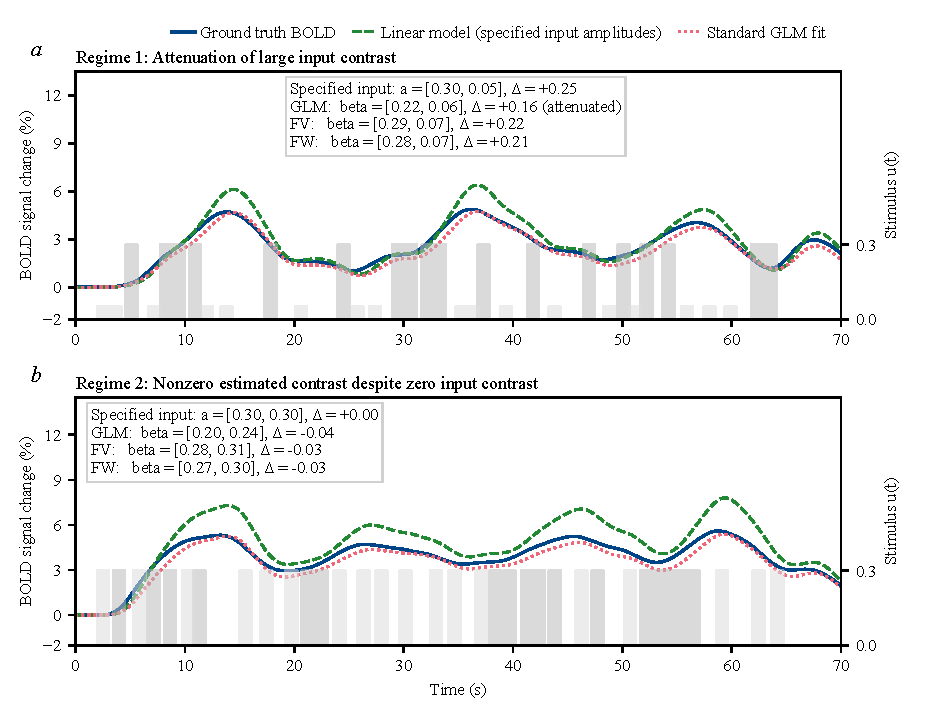
\includegraphics[width=16cm]{fig_4}
	\caption{Два режима нелинейного искажения BOLD-сигнала в последовательностях стимулов: \textit{a} --- занижение контраста при $a_A=0{,}30$, $a_B=0{,}05$ и пуассоновском предъявлении стимулов со средним SOA 1,7~с; \textit{b} --- ненулевая оценка контраста при равных амплитудах $a_A=a_B=0{,}30$ и нулевом заданном контрасте, когда условие A предъявляется с короткими интервалами, а B с более длинными. Сплошная синяя линия --- BOLD-отклик P-DCM, серые столбики на правой оси --- моменты предъявления стимулов условий A и B, зеленый штрих --- линейная модель с канонической HRF при входных амплитудах, красный пунктир --- стандартная оценка ОЛМ; в надписях на панелях --- оценки коэффициентов и контраста для ОЛМ и поправок FV и FW. Запись 70~с, длительность стимула 1~с.}
	\label{fig:f4}
\end{figure}

\subsection*{Форма HRF и ошибка конечных амплитуд}

Собственное линейное приближение проверялось в пределе слабого сигнала: при пиковом приросте потока $0{,}01$ относительная норма $L^2$ разности полного и собственного линейного ответов составляет $0{,}2\%$ и $0{,}3\%$ для P-DCM и BW соответственно. Линейный отклик номинальной P-DCM близок к канонической HRF по положению пика и глубине постстимульного снижения (рис.~\ref{fig:f1}). У BW максимум заметно позже и снижение глубже. 

Однако точность линейного приближения и близость форм не гарантируют точность оценок при конечных амплитудах.
При $L_1$ ошибка контраста сохраняется и растет с амплитудой (рис.~\ref{fig:f5}, табл.~\ref{tab:amp}). В амплитудной бесшумной серии при $a_A=0{,}025$ медианная относительная ошибка у обоих генераторов составляет единицы процентов, а при $a_A=0{,}2$ в последовательностях со средним SOA 2~с достигает четверти контраста. С ростом интервала ошибка уменьшается, но все еще заметна и при SOA 8~с. 

\begin{figure}[!ht]
	\centering
	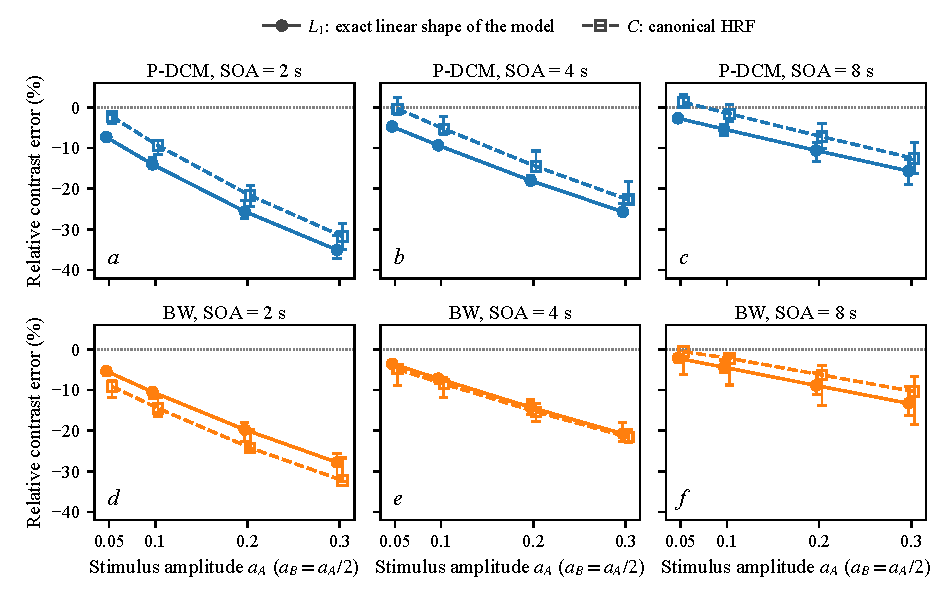
\includegraphics[width=16cm]{fig_5}
	\caption{Относительная ошибка контраста $100(\hat\Delta-\Delta)/\Delta$ при использовании собственного линейного ядра $L_1$ для P-DCM и BW в зависимости от $a_A$ при $a_B=a_A/2$. Рисунки \textit{a}, \textit{b} и \textit{c} соответствуют средним SOA 2, 4 и 8~с; маркеры --- медианы трех последовательностей стимулов, полосы --- описательный разброс min--max между ними.}
	\label{fig:f5}
\end{figure}

\begin{table}[!t]
\captionsetup{justification=raggedright}
\caption{Относительная ошибка контраста: медиана и разброс min--max по последовательностям стимулов; <<все>> --- по девяти последовательностям, отдельные SOA --- по трем последовательностям данного среднего; в амплитудной серии $a_B=0{,}5a_A$, в механистической --- $a_B=0{,}025$}
\label{tab:amp}
\centering
\small
\setlength{\tabcolsep}{4pt}
\begin{tabular}{clccccccc}
\hline
\multirow{2}{*}{$a_A$} & \multirow{2}{*}{SOA} & \multirow{2}{*}{Оценка} & \multicolumn{3}{c}{P-DCM, \%} & \multicolumn{3}{c}{BW, \%}\\
\cline{4-9}
 & & & медиана & min & max & медиана & min & max\\
\hline
\multicolumn{9}{r}{\rule{0pt}{12pt}\itshape Амплитудная серия}\\[2pt]
$0{,}025$ & все & $L_1$ & $-2{,}5$ & $-4{,}3$ & $-1{,}0$ & $-1{,}8$ & $-3{,}1$ & $-0{,}6$\\[2pt]
\hline
\rule[-2pt]{0pt}{14pt}\multirow{4}{*}{$0{,}2$} & 2~с & \multirow{3}{*}{$L_1$} & $-25{,}4$ & $-29{,}6$ & $-23{,}7$ & $-19{,}9$ & $-23{,}0$ & $-16{,}3$\\
 & 4~с & & $-18{,}2$ & $-20{,}9$ & $-15{,}1$ & $-14{,}0$ & $-17{,}2$ & $-10{,}9$\\
 & 8~с & & $-9{,}1$ & $-11{,}2$ & $-7{,}9$ & $-7{,}3$ & $-9{,}3$ & $-5{,}4$\\[2pt]
\cline{2-9}
 & \rule[-2pt]{0pt}{14pt}все & $C$ & $-14{,}5$ & $-24{,}5$ & $-4{,}0$ & $-15{,}3$ & $-24{,}9$ & $-4{,}0$\\[2pt]
\hline
\rule[-2pt]{0pt}{14pt}$0{,}3$ & все & $C$ & $-22{,}7$ & $-34{,}9$ & $-8{,}6$ & $-21{,}6$ & $-32{,}5$ & $-6{,}8$\\[2pt]
\multicolumn{9}{r}{\rule{0pt}{12pt}\itshape Механистическая серия}\\[2pt]
\multirow{2}{*}{$0{,}05$} & \multirow{2}{*}{все} & $C$ & $-0{,}3$ & $-4{,}0$ & $+3{,}1$ & $-6{,}2$ & $-11{,}9$ & $-0{,}2$\\
 & & $L_1$ & $-4{,}7$ & $-7{,}9$ & $-2{,}0$ & $-3{,}5$ & $-6{,}3$ & $-1{,}2$\\
\hline
\end{tabular}
\end{table}

\subsection*{Общий уровень стимуляции и история условий}

Одна и та же разность амплитуд дает разную ошибку контраста в зависимости от общего уровня стимуляции $m=(a_A+a_B)/2$ (средней амплитуды входного воздействия). В механистической серии контраст удерживался равным $0{,}1$, а обе амплитуды росли от пары $(0{,}15;\,0{,}05)$ до пары $(0{,}30;\,0{,}20)$. Медианная ошибка $C$ выросла по модулю втрое у P-DCM и почти вдвое у BW; полные разбросы показаны на рис.~\ref{fig:f6}, \textit{c}.

Разметка событий способна сама по себе создавать ненулевую оценку контраста (рис.~\ref{fig:f6}, \textit{d}). При равных амплитудах и нулевом заданном контрасте события разных меток попадали в разные гемодинамические контексты: стимулы условия A шли на фоне недавних ответов, а одиночные события B следововали после более длительного восстановления сосудистого состояния. Линейная модель относила часть этого различия к коэффициентам условий.

Полная квадратичная проекция точнее статической при $a_A\le0{,}1$ у обоих генераторов. У BW это верно во всем показанном диапазоне амплитуд, а у P-DCM при $a_A=0{,}2$ и $0{,}3$ полная проекция завышает модуль ошибки, и статическая оказывается точнее.

\begin{figure}[!t]
	\centering
	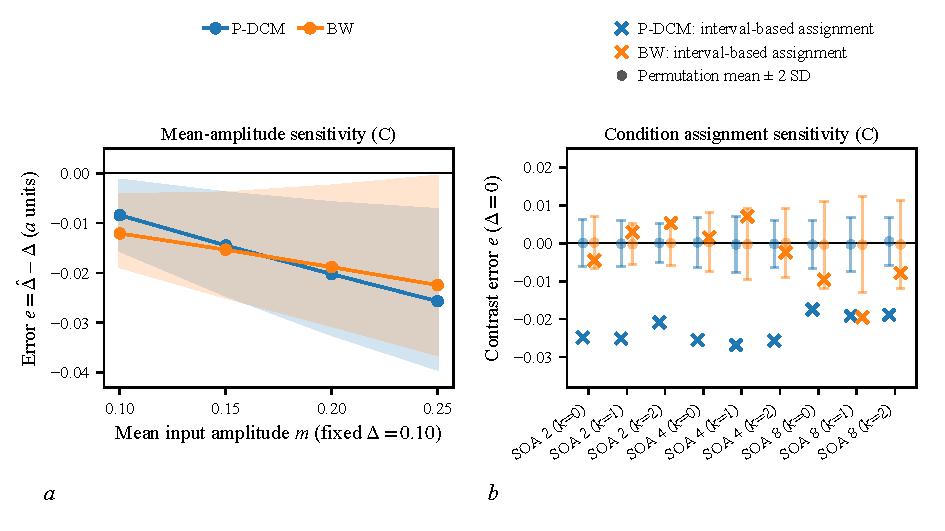
\includegraphics[width=15.5cm]{fig_6}
	\caption{Механизмы ошибки контраста для P-DCM и BW. \textit{a} --- медиана ошибки $e=\hat\Delta-\Delta$ по девяти последовательностям стимулов для $C$ и собственного $L_1$ при $a_B=a_A/2$; пунктир --- $\pm0{,}002$ модельной единицы. \textit{b} --- компоненты ошибки, предсказанные приближением второго порядка: фактическая нелинейная ошибка $e_{\mathrm{nl}}$, полная и статическая проекции. \textit{c} --- ошибка $C$ при росте средней амплитуды входного воздействия $m=(a_A+a_B)/2$ и фиксированном $\Delta=0{,}10$; полосы --- разброс min--max. \textit{d} --- ошибка $C$ при $a_A=a_B=0{,}20$ и $\Delta=0$: метки по истории событий и среднее $\pm2$ стандартных отклонения по 100 перестановкам; $k$ --- номер последовательности при данном среднем SOA. Обозначения на панелях: L1own --- собственное $L_1$, full Q --- полная квадратичная проекция, static Q --- статическая проекция.}
	\label{fig:f6}
\end{figure}

\subsection*{Полная поправка Вольтерра второго порядка}

Чтобы считать применение FV обоснованным, были заданы два условия: общее снижение RMSE контраста не менее $0{,}002$ и ухудшение в отдельном варианте условий не более $0{,}001$. Первое условие было выполнено: абсолютная RMSE уменьшилась на $\approx0{,}003$ (рис.~\ref{fig:f7}, \textit{a}). В основном классе ненулевых контрастов относительная RMSE снизилась с $28{,}7$ до $25{,}0\%$. Наибольшее снижение ошибки (примерно втрое) зафиксировано при среднем SOA 2~с. В единственной паре малого контраста $(0{,}2;\,0{,}18)$ применение FV увеличило ошибку: $53{,}1\%$ против $50{,}3\%$.

Второе условие не было выполнено: при изменении выходного усиления (рис.~\ref{fig:f7}, \textit{b}) в 40 тестовых последовательностях со средним SOA 8~с и усилениями $0{,}8$ и $1{,}25$ FV увеличила RMSE контраста во всех трех классах контраста. Этот результат получен прямым расчетом ожидания по известному распределению шума и не зависит от приближенных интервалов.

\begin{figure}[!t]
	\centering
	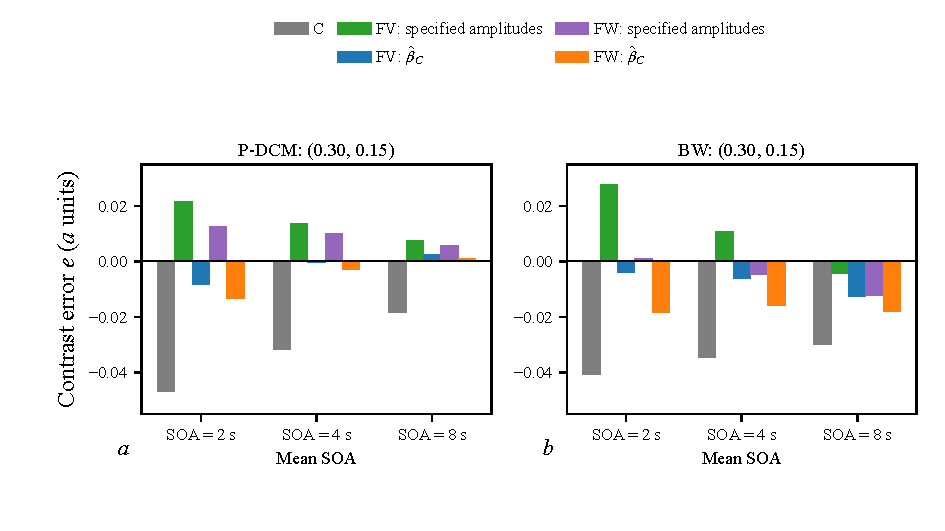
\includegraphics[width=16cm]{fig_7}
	\caption{Тестирование поправки FV: сводная RMSE и ухудшение по вариантам. \textit{a} --- RMSE контраста для $C$ и FV по четырем заранее заданным режимам и по всей совокупности. \textit{b} --- точечные оценки ухудшения точности $H_R=R_{\mathrm{FV}}-R_C$ и односторонние верхние границы для 36 заранее определенных вариантов (четыре режима, три класса контраста, три средних SOA); индексы 0--8, 9--17, 18--26 и 27--35 отвечают режимам Gain, Nominal, Parameter и Structure. Группа проходит условие, пока верхняя граница $H_R$ остается ниже красной линии --- допуска $0{,}001$. Верхние границы построены бутстрепом по последовательностям стимулов (1000 бутстреп-выборок) с нормальной аппроксимацией и поправкой Бонферрони при $\alpha=0{,}05$; $R$ --- RMSE контраста.}
	\label{fig:f7}
\end{figure}

\subsection*{Роль выходного усиления}

При выходном усилении $g$ заданный контраст $\Delta=a_A-a_B$ остается в исходной шкале. Линейные оценки меняются пропорционально $g$. Квадратичный вклад, вычисленный по оцененному входу, меняется пропорционально квадрату оценок, поэтому номинальная и фактическая нелинейность масштабируются по-разному. Диагностическим эталоном служит произведение усиления на заданный контраст, $g\Delta$. Этот эталон отделяет рассогласование выходной шкалы от нелинейного сжатия: ошибка относительно него равна $e_g=\hat\Delta-g\Delta=e-(g-1)\Delta$. Снижение ошибки относительно $g\Delta$ означает согласование с выходной шкалой, но при неизвестном $g$ модельную шкалу не восстанавливает: ошибка относительно $\Delta$ сохраняется.

Для режима $g=1{,}25$ и основного класса контрастов FV снизила RMSE относительно эталона $g\Delta$ примерно на три четверти: на $75{,}8\%$ без шума и на $76{,}0\%$ при SNR~8. При SNR~2 устойчивого улучшения нет.

\subsection*{Статическая поправка винеровского типа}

FW улучшала отдельные коэффициенты чаще, чем их разность, а подтвержденное улучшение контраста было достигнуто в меньшинстве вариантов (табл.~\ref{tab:fw}). Тестирование FW охватило 288 вариантов условий: сочетания генератора, варианта поправки (собственного или перенесенного), усиления, среднего SOA, амплитуд и уровня шума. В 144 вариантах без изменения усиления улучшение контраста подтверждено только в 28, причем во всех осталось частичным: после поправки ошибки не вошли в порог. В 102 вариантах порога не достигла ни одна из оценок, в остальных оценка с $C$ была достаточной до поправки либо исходы остались неразличимыми (табл.~\ref{tab:fw}). 

\begin{table}[h]
\caption{Распределение 144 вариантов без изменения усиления тестирования поправки FW по исходам для коэффициентов $\beta$ и контраста $A-B$. В скобках указано число вариантов с полным улучшением. Порог приемлемой ошибки $\delta_s=\max(0{,}002;\,0{,}05m_s)$ определен по масштабу $m_s$ каждого варианта}
\label{tab:fw}
\centering
\begin{tabular}{lcc}
\hline
Исход & Коэффициенты & Контраст $A-B$\\
\hline
Оценка с $C$ достаточна & 10 & 12\\
Улучшение подтверждено & 84 (8) & 28 (0)\\
Порог не достигнут ни одной оценкой & 43 & 102\\
Исходы не различимы & 7 & 2\\
\hline
\end{tabular}
\end{table}

В среднем по всем 288 вариантам FW почти не меняла ошибку коэффициентов: среднеквадратичная относительная ошибка оценок $\hat\beta_A$ и $\hat\beta_B$ составляет $25{,}3\%$ у $C$ и $25{,}2\%$ у FW. На всех уровнях шума различие между $C$ и FW не превышает $0{,}5$ процентного пункта, а при SNR~2 сама ошибка достигает трети амплитуды. В рассмотренных модельных условиях с высоким уровнем шума (SNR~2) FW не улучшала активационные оценки: улучшение контраста не подтверждено ни в одном из 96 вариантов. То же в вариантах малых амплитуд и в 72 вариантах с усилением $1{,}25$.

\subsection*{Границы второго порядка и оцененного входа}

Поправки FV и FW вычитают ошибку, предсказанную приближением второго порядка, поэтому их точность упирается в точность этого приближения. Приближение верно воспроизводит знак ошибки контраста всюду, где он различим, и ее величину примерно в двух третях случаев. Для каждого из двух генераторов проверено 45 сочетаний амплитуд, SOA и последовательностей стимулов, всего 90 сочетаний (рис.~\ref{fig:f8}). Знак считался различимым при абсолютной ошибке $0{,}002$ и выше одновременно в теоретическом и полном расчете. Таких сочетаний 67, и во всех знаки совпали. Критерий близости величины (расхождение не более $25\%$) выполнен в 62 из 90 случаев.

Предел приближения виден у P-DCM при $a_A=0{,}3$, $a_B=0{,}15$ и среднем SOA 2~с. Предсказание второго порядка составляет $-0{,}0615$ модельной единицы, фактическая ошибка полного генератора равна $-0{,}0468$. Остаток $+0{,}0147$ частично компенсирует квадратичный вклад, поэтому при сильной стимуляции предсказание завышает модуль нелинейной ошибки.

\begin{figure}[!ht]
	\centering
	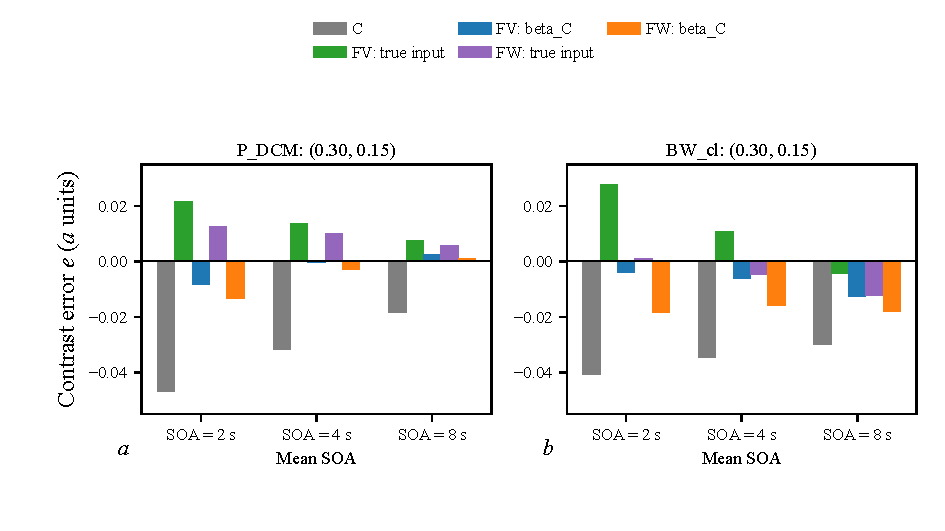
\includegraphics[width=16cm]{fig_8}
	\caption{Ошибки контраста $e=\hat\Delta-\Delta$ при $a_A=0{,}30$, $a_B=0{,}15$, основной последовательности ($k=0$) и средних SOA 2, 4 и 8~с для P-DCM (\textit{a}) и BW (\textit{b}). Столбцы --- каноническая оценка $C$, поправки FV и FW с входными амплитудами (теоретический контроль; при анализе реальных данных входные амплитуды неизвестны) и те же поправки с подстановкой оценок $\hat\beta_C$; обозначение beta\_C в легенде соответствует $\hat\beta_C$. Отдельная бесшумная диагностическая серия; со сводным тестированием FV и таблицей исходов FW она не объединяется.}
	\label{fig:f8}
\end{figure}

% !TeX root = ../main.tex

\section{Обсуждение}

Бета-коэффициенты ОЛМ нельзя без дополнительных предпосылок считать прямым измерением силы нейронального ответа: они зависят от входного воздействия, гемодинамического преобразования, выбранной HRF и временной структуры исследования. Вычитание коэффициентов устраняет только общий аддитивный фон. Общий множитель сохраняется в масштабе контраста, а при нелинейном преобразовании ошибка зависит еще и от самих амплитуд. Это видно уже из зависимости $b(a)=a-\eta a^2$ с $\eta>0$: разность выходов равна $(a_A-a_B)[1-\eta(a_A+a_B)]=\Delta(1-2\eta m)$ и при неизменной разности амплитуд меняется с общим уровнем $m$ (ср. рис.~\ref{fig:f6}, \textit{c}). В динамической системе добавляется влияние предыстории: последовательность предъявления стимулов определяет состояние генератора и проекцию нелинейного остатка на коэффициенты условий. Поэтому конкретная последовательность событий важна не меньше средней частоты предъявления.

Точное линейное ядро и точная оценка конечной амплитуды решают разные задачи. $L_1$ описывает чувствительность модели около покоя, но не обязано минимизировать ошибки $\beta$ и контраста при конечном входе. Если проекция ошибки канонической формы противоположна нелинейному вкладу, оценка может оказаться ближе к заданному значению, однако такая компенсация зависит от амплитуд и последовательности предъявления стимулов. По той же причине хорошее воспроизведение BOLD-ряда не обеспечивает точность активационных оценок: расхождение сигнала и его проекция на выбранный контраст являются разными величинами.

Поправка второго порядка ограничена локальностью разложения и ошибкой оцененного входа. При росте амплитуды увеличивается роль высших порядков, поэтому правильное вычисление $Q_0$ не гарантирует правильную величину поправки. Если исходные оценки занижены, $\hat u_C$ описывает иную силу воздействия; если они содержат шум, квадратичное преобразование меняет и разброс, и среднее. Даже при нулевом среднем ошибки ее квадрат имеет положительное среднее; это известное смещение подстановочных оценок квадратичных функционалов~\cite{butucea2011}.

Две другие причины ухудшения точности связаны со шкалой наблюдения и несоответствием модели. При неизвестном выходном усилении номинальная и фактическая нелинейность масштабируются по-разному (подраздел <<Роль выходного усиления>>), что и проявилось при усилениях $0{,}8$ и $1{,}25$. Кроме того, номинальная модель может отличаться от генератора по параметрам или структуре. Сопоставление P-DCM и BW проверяет эту чувствительность, но не позволяет выбрать физиологически верное описание.

Результаты согласуются с представлением о BOLD как отклике нелинейной гемодинамической системы~\cite{friston2000,buxton2004} и с ролью нейрональных и сосудистых переходных процессов~\cite{havlicek2015}. Зависимость оценок от истории стимуляции отмечалась и в предшествующих работах~\cite{wager2005}. В настоящей работе количественно проверены канонические оценки и фиксированные поправки в проверенной модельной области. Использование собственного $L_1$ делает явным источник ошибки: видно, какая часть занижения остается после устранения рассогласования формы.

Систематическая составляющая ошибки важна и при усреднении индивидуальных оценок. Хотя групповое исследование не проводилось, из модели $\hat\Delta_i=\Delta_i+b_i+\varepsilon_i$ с независимым шумом нулевого среднего следуют два вывода. Смещение среднего равно $N^{-1}\sum_i b_i$, поэтому общий систематический сдвиг $b_i=b$ усреднением не уменьшается. Дисперсия шумовой части при одинаковой $\sigma^2$ составляет $\sigma^2/N$; если шумовые составляющие разных участников коррелированы, темп $1/\sqrt N$ не гарантирован. Усреднение индивидуально скорректированных оценок и поправка после усреднения BOLD являются разными операциями; эти аналитические следствия не заменяют групповую проверку.

Полученные данные не задают единого безопасного интервала между стимулами: для такого вывода нужно заранее определить допустимые ошибки $\beta$ и контраста, амплитуды, длительности, параметры генератора и правила агрегирования. Уменьшение ошибки при среднем SOA 8~с в рассмотренных сериях не устанавливает универсального порога 8~с для фМРТ. Уменьшение ошибок в одних условиях также не означает, что поправка безопасна в других; полезные группы, выделенные после теста, остаются описательными.

Генераторы имеют заданные параметры и не описывают пространственную структуру сосудистой сети, а общий линейный E/I-блок исключает нелинейную нейрональную адаптацию, которая может присутствовать в физиологических данных. Близость номинальной P-DCM к $C$ относится к конкретным параметрам. Переход к BW меняет несколько элементов сразу, поэтому различия результатов не идентифицируют единственный механизм.

Основные выводы получены для секундных событий и выбранных амплитуд. Блоковые дизайны и события другой длительности не исследовались, а отдельные серии используют разные последовательности предъявления стимулов и процедуры и не образуют единой проверенной поверхности. Поэтому численные границы нельзя переносить на другие дизайны без дополнительной проверки.

В шумовых сериях ковариация считалась известной, ее оценивание по данным не проверялось. Восемь повторов не дают точной оценки условных смещений, интервалы приближенные; мощность и частота ложных решений не исследованы. Независимой реализации внешним исследователем не было. Отрицательный итог FV на ее области не переносится автоматически на FW, а частные улучшения FW не отменяют ограничения FV.

% !TeX root = ../main.tex


\section*{Заключение}

Стандартная оценка контраста с канонической HRF при нелинейной гемодинамике смещена, и смещение зависит от амплитуд, плотности и последовательности событий. Собственное линейное ядро генератора устраняет лишь ошибку формы HRF и этого смещения не снимает, поскольку нелинейный вклад остается. Несовпадение канонической формы может как усиливать, так и частично компенсировать нелинейный вклад, поэтому близость форм сама по себе точности не гарантирует.

Ранее нелинейность BOLD-отклика подтверждалась качественно, по соответствию модельных кривых наблюдаемому сигналу. В настоящей работе ошибки активационных оценок вычислены против точного эталона и разложены на вклад формы HRF, нелинейной динамики и шума, а границы применимости линейного анализа и фиксированных поправок определены количественно, по заранее заданным порогам. Приближение второго порядка верно воспроизводит знак ошибки контраста и потому пригодно для диагностики ее направления.

Для практики это означает, что при плотных последовательностях событий контраст нельзя рассматривать как прямую меру разности амплитуд воздействия, а различия в последовательностях предшествующих событий способны давать ненулевую оценку при равных амплитудах. Численные границы относятся к исследованным моделям и протоколам, их перенос на данные человека требует отдельного обоснования.


%%%%%%%%%%%%%%%%%%%%%%%%%%%%%%%%%%%%%%%%%%%%%%%%%%%%%%%%%%%%%%%%%%%%%%%%%%%%%%%

% !TeX root = ../main.tex

% Библиографический список
\begin{ltrtr}

	\bibitem{ogawa1990}
	\textit{Ogawa~S., Lee~T.\,M., Kay~A.\,R., Tank~D.\,W.} Brain magnetic resonance imaging with contrast dependent on blood oxygenation~// Proc. Natl. Acad. Sci. USA. 1990. Vol.~87, no.~24. P.~9868--9872. \href{https://doi.org/10.1073/pnas.87.24.9868}{DOI:~10.1073/\allowbreak pnas.87.24.9868}.

	\bibitem{kwong1992}
	\textit{Kwong~K.\,K., Belliveau~J.\,W., Chesler~D.\,A., et al.} Dynamic magnetic resonance imaging of human brain activity during primary sensory stimulation~// Proc. Natl. Acad. Sci. USA. 1992. Vol.~89, no.~12. P.~5675--5679. \href{https://doi.org/10.1073/pnas.89.12.5675}{DOI:~10.1073/\allowbreak pnas.89.12.5675}.

	\bibitem{kireev2013}
	\textit{Киреев~М.\,В., Захс~Д.\,В., Коротков~А.\,Д., Медведев~С.\,В.} Современные методы функциональной томографической нейровизуализации в исследовании функций больного и здорового мозга~// Рос. физиол. журн. им. И.\,М. Сеченова. 2013. Т.~99, №~1. С.~53--62.

	\bibitem{myznikov2026}
	\textit{Мызников~А.\,Д., Селиверстов~Р.\,Ю., Коротков~А.\,Д., Алиев~Г.\,Б., Чередниченко~Д.\,В., Дидур~М.\,Д., Киреев~М.\,В.} Негативный BOLD-сигнал как способ комплиментарной характеристики мозгового обеспечения функций: потенциал использования в предхирургической подготовке методом функциональной магнитно-резонансной томографии~// Рос. физиол. журн. им. И.\,М. Сеченова. 2026. Т.~112, №~6. С.~1337--1373. \href{https://doi.org/10.7868/S2658655X26060014}{DOI:~10.7868/\allowbreak S2658655X26060014}.

	\bibitem{friston2000}
	\textit{Friston~K.\,J., Mechelli~A., Turner~R., Price~C.\,J.} Nonlinear responses in fMRI: the Balloon model, Volterra kernels, and other hemodynamics~// NeuroImage. 2000. Vol.~12, no.~4. P.~466--477. \href{https://doi.org/10.1006/nimg.2000.0630}{DOI:~10.1006/\allowbreak nimg.2000.0630}.

	\bibitem{buxton2004}
	\textit{Buxton~R.\,B., Uludag~K., Dubowitz~D.\,J., Liu~T.\,T.} Modeling the hemodynamic response to brain activation~// NeuroImage. 2004. Vol.~23, Suppl.~1. P.~S220--S233. \href{https://doi.org/10.1016/j.neuroimage.2004.07.013}{DOI:~10.1016/\allowbreak j.neuroimage.2004.07.013}.

	\bibitem{mandeville1999}
	\textit{Mandeville~J.\,B., Marota~J.\,J.\,A., Ayata~C., et al.} Evidence of a cerebrovascular postarteriole windkessel with delayed compliance~// J. Cereb. Blood Flow Metab. 1999. Vol.~19, no.~6. P.~679--689. \href{https://doi.org/10.1097/00004647-199906000-00012}{DOI:~10.1097/\allowbreak 00004647-\allowbreak 199906000-\allowbreak 00012}.

	\bibitem{masharipov2025}
	\textit{Машарипов~Р.\,С., Дидур~М.\,Д., Чередниченко~Д.\,В., Киреев~М.\,В.} Изучение контекстно-зависимых функциональных связей с помощью функциональной магнитно-резонансной томографии~// Журн. высш. нервн. деят. им. И.\,П. Павлова. 2025. Т.~75, №~5. С.~530--552. \href{https://doi.org/10.31857/S0044467725050037}{DOI:~10.31857/\allowbreak S0044467725050037}.

	\bibitem{friston1998b}
	\textit{Friston~K.\,J., Fletcher~P., Josephs~O., et al.} Event-related fMRI: characterizing differential responses~// NeuroImage. 1998. Vol.~7, no.~1. P.~30--40. \href{https://doi.org/10.1006/nimg.1997.0306}{DOI:~10.1006/\allowbreak nimg.1997.0306}.

	\bibitem{friston1994}
	\textit{Friston~K.\,J., Holmes~A.\,P., Worsley~K.\,J., et al.} Statistical parametric maps in functional imaging: a general linear approach~// Hum. Brain Mapp. 1994. Vol.~2, no.~4. P.~189--210. \href{https://doi.org/10.1002/hbm.460020402}{DOI:~10.1002/\allowbreak hbm.460020402}.

	\bibitem{medvedev2012}
	\textit{Медведев~С.\,В., Киреев~М.\,В., Коротков~А.\,Д.} Функциональная МРТ и ПЭТ в клинической практике~--- общие принципы и ограничения при картировании функций мозга~// Лучевая диагностика и терапия. 2012. №~3(3). С.~20--26.

	\bibitem{monti2011}
	\textit{Monti~M.\,M.} Statistical analysis of fMRI time-series: a critical review of the GLM approach~// Front. Hum. Neurosci. 2011. Vol.~5. P.~28. \href{https://doi.org/10.3389/fnhum.2011.00028}{DOI:~10.3389/\allowbreak fnhum.2011.00028}.

	\bibitem{handwerker2012}
	\textit{Handwerker~D.\,A., Gonzalez-Castillo~J., D'Esposito~M., Bandettini~P.\,A.} The continuing challenge of understanding and modeling hemodynamic variation in fMRI~// NeuroImage. 2012. Vol.~62, no.~2. P.~1017--1023. \href{https://doi.org/10.1016/j.neuroimage.2012.02.015}{DOI:~10.1016/\allowbreak j.neuroimage.2012.02.015}.

	\bibitem{lindquist2009}
	\textit{Lindquist~M.\,A., Meng Loh~J., Atlas~L.\,Y., Wager~T.\,D.} Modeling the hemodynamic response function in fMRI: efficiency, bias and mis-modeling~// NeuroImage. 2009. Vol.~45, no.~1, Suppl.~1. P.~S187--S198. \href{https://doi.org/10.1016/j.neuroimage.2008.10.065}{DOI:~10.1016/\allowbreak j.neuroimage.2008.10.065}.

	\bibitem{polimeni2021}
	\textit{Polimeni~J.\,R., Lewis~L.\,D.} Imaging faster neural dynamics with fast fMRI: a need for updated models of the hemodynamic response~// Prog. Neurobiol. 2021. Vol.~207. P.~102174. \href{https://doi.org/10.1016/j.pneurobio.2021.102174}{DOI:~10.1016/\allowbreak j.pneurobio.2021.102174}.

	\bibitem{woolrich2004}
	\textit{Woolrich~M.\,W., Behrens~T.\,E.\,J., Smith~S.\,M.} Constrained linear basis sets for HRF modelling using Variational Bayes~// NeuroImage. 2004. Vol.~21, no.~4. P.~1748--1761. \href{https://doi.org/10.1016/j.neuroimage.2003.12.024}{DOI:~10.1016/\allowbreak j.neuroimage.2003.12.024}.

	\bibitem{wager2003}
	\textit{Wager~T.\,D., Nichols~T.\,E.} Optimization of experimental design in fMRI: a general framework using a genetic algorithm~// NeuroImage. 2003. Vol.~18, no.~2. P.~293--309. \href{https://doi.org/10.1016/S1053-8119(02)00046-0}{DOI:~10.1016/\allowbreak S1053-\allowbreak 8119(02)00046-\allowbreak 0}.

	\bibitem{friston1998}
	\textit{Friston~K.\,J., Josephs~O., Rees~G., Turner~R.} Nonlinear event-related responses in fMRI~// Magn. Reson. Med. 1998. Vol.~39, no.~1. P.~41--52. \href{https://doi.org/10.1002/mrm.1910390109}{DOI:~10.1002/\allowbreak mrm.1910390109}.

	\bibitem{robinson2006}
	\textit{Robinson~P.\,A., Drysdale~P.\,M., Van der Merwe~H., et al.} BOLD responses to stimuli: dependence on frequency, stimulus form, amplitude, and repetition rate~// NeuroImage. 2006. Vol.~31, no.~2. P.~585--599. \href{https://doi.org/10.1016/j.neuroimage.2005.12.026}{DOI:~10.1016/\allowbreak j.neuroimage.2005.12.026}.

	\bibitem{birn2001}
	\textit{Birn~R.\,M., Saad~Z.\,S., Bandettini~P.\,A.} Spatial heterogeneity of the nonlinear hemodynamic response~// NeuroImage. 2001. Vol.~14, no.~4. P.~817--826. \href{https://doi.org/10.1006/nimg.2001.0873}{DOI:~10.1006/\allowbreak nimg.2001.0873}.

	\bibitem{mechelli2001}
	\textit{Mechelli~A., Price~C.\,J., Friston~K.\,J.} Nonlinear coupling between evoked rCBF and BOLD signals: a simulation study of hemodynamic responses~// NeuroImage. 2001. Vol.~14, no.~4. P.~862--872. \href{https://doi.org/10.1006/nimg.2001.0876}{DOI:~10.1006/\allowbreak nimg.2001.0876}.

	\bibitem{magri2011}
	\textit{Magri~C., Logothetis~N.\,K., Panzeri~S.} Investigating static nonlinearities in neurovascular coupling~// Magn. Reson. Imaging. 2011. Vol.~29, no.~10. P.~1358--1364. \href{https://doi.org/10.1016/j.mri.2011.04.017}{DOI:~10.1016/\allowbreak j.mri.2011.04.017}.

	\bibitem{buxton1998}
	\textit{Buxton~R.\,B., Wong~E.\,C., Frank~L.\,R.} Dynamics of blood flow and oxygenation changes during brain activation: the Balloon model~// Magn. Reson. Med. 1998. Vol.~39, no.~6. P.~855--864. \href{https://doi.org/10.1002/mrm.1910390602}{DOI:~10.1002/\allowbreak mrm.1910390602}.

	\bibitem{friston2003}
	\textit{Friston~K.\,J., Harrison~L., Penny~W.} Dynamic causal modelling~// NeuroImage. 2003. Vol.~19, no.~4. P.~1273--1302. \href{https://doi.org/10.1016/S1053-8119(03)00202-7}{DOI:~10.1016/\allowbreak S1053-\allowbreak 8119(03)00202-\allowbreak 7}.

	\bibitem{wager2005}
	\textit{Wager~T.\,D., Vazquez~A., Hernandez~L., Noll~D.\,C.} Accounting for nonlinear BOLD effects in fMRI: parameter estimates and a model for prediction in rapid event-related studies~// NeuroImage. 2005. Vol.~25, no.~1. P.~206--218. \href{https://doi.org/10.1016/j.neuroimage.2004.11.008}{DOI:~10.1016/\allowbreak j.neuroimage.2004.11.008}.

	\bibitem{welvaert2014}
	\textit{Welvaert~M., Rosseel~Y.} A review of fMRI simulation studies~// PLoS ONE. 2014. Vol.~9, no.~7. P.~e101953. \href{https://doi.org/10.1371/journal.pone.0101953}{DOI:~10.1371/\allowbreak journal.pone.0101953}.

	\bibitem{ellis2020}
	\textit{Ellis~C.\,T., Baldassano~C., Schapiro~A.\,C., Cai~M.\,B., Cohen~J.\,D.} Facilitating open-science with realistic fMRI simulation: validation and application~// PeerJ. 2020. Vol.~8. P.~e8564. \href{https://doi.org/10.7717/peerj.8564}{DOI:~10.7717/\allowbreak peerj.8564}.

	\bibitem{cakan2023}
	\textit{Cakan~C., Jajcay~N., Obermayer~K.} neurolib: a simulation framework for whole-brain neural mass modeling~// Cogn. Comput. 2023. Vol.~15, no.~4. P.~1132--1152. \href{https://doi.org/10.1007/s12559-021-09931-9}{DOI:~10.1007/\allowbreak s12559-\allowbreak 021-\allowbreak 09931-\allowbreak 9}.

	\bibitem{havlicek2015}
	\textit{Havlicek~M., Roebroeck~A., Friston~K., Gardumi~A., Ivanov~D., Uludag~K.} Physiologically informed dynamic causal modeling of fMRI data~// NeuroImage. 2015. Vol.~122. P.~355--372. \href{https://doi.org/10.1016/j.neuroimage.2015.07.078}{DOI:~10.1016/\allowbreak j.neuroimage.2015.07.078}.

	\bibitem{sanzleon2015}
	\textit{Sanz-Leon~P., Knock~S.\,A., Spiegler~A., Jirsa~V.\,K.} Mathematical framework for large-scale brain network modeling in The Virtual Brain~// NeuroImage. 2015. Vol.~111. P.~385--430. \href{https://doi.org/10.1016/j.neuroimage.2015.01.002}{DOI:~10.1016/\allowbreak j.neuroimage.2015.01.002}.

	\bibitem{deneux2006}
	\textit{Deneux~T., Faugeras~O.} Using nonlinear models in fMRI data analysis: model selection and activation detection~// NeuroImage. 2006. Vol.~32, no.~4. P.~1669--1689. \href{https://doi.org/10.1016/j.neuroimage.2006.03.006}{DOI:~10.1016/\allowbreak j.neuroimage.2006.03.006}.

	\bibitem{volterra1930}
	\textit{Volterra~V.} Theory of Functionals and of Integral and Integro-Differential Equations. London: Blackie and Son, 1930.

	\bibitem{schetzen1980}
	\textit{Schetzen~M.} The Volterra and Wiener Theories of Nonlinear Systems. New York: Wiley, 1980.

	\bibitem{marmarelis2004}
	\textit{Marmarelis~V.\,Z.} Nonlinear Dynamic Modeling of Physiological Systems. Hoboken: IEEE Press; Wiley-Interscience, 2004. \href{https://doi.org/10.1002/9780471679370}{DOI:~10.1002/\allowbreak 9780471679370}.

	\bibitem{hunter1986}
	\textit{Hunter~I.\,W., Korenberg~M.\,J.} The identification of nonlinear biological systems: Wiener and Hammerstein cascade models~// Biol. Cybern. 1986. Vol.~55, no.~2--3. P.~135--144. \href{https://doi.org/10.1007/BF00341929}{DOI:~10.1007/\allowbreak BF00341929}.

	\bibitem{boyd1985}
	\textit{Boyd~S., Chua~L.\,O.} Fading memory and the problem of approximating nonlinear operators with Volterra series~// IEEE Trans. Circuits Syst. 1985. Vol.~32, no.~11. P.~1150--1161. \href{https://doi.org/10.1109/TCS.1985.1085649}{DOI:~10.1109/\allowbreak TCS.1985.1085649}.

	\bibitem{pintelon2012}
	\textit{Pintelon~R., Schoukens~J.} System Identification: A Frequency Domain Approach. 2nd ed. Hoboken: Wiley, 2012. \href{https://doi.org/10.1002/9781118287422}{DOI:~10.1002/\allowbreak 9781118287422}.

	\bibitem{schoukens2015}
	\textit{Schoukens~J., Pintelon~R., Rolain~Y., et al.} Structure discrimination in block-oriented models using linear approximations: a theoretic framework~// Automatica. 2015. Vol.~53. P.~225--234. \href{https://doi.org/10.1016/j.automatica.2014.12.045}{DOI:~10.1016/\allowbreak j.automatica.2014.12.045}.

	\bibitem{glover1999}
	\textit{Glover~G.\,H.} Deconvolution of impulse response in event-related BOLD fMRI~// NeuroImage. 1999. Vol.~9, no.~4. P.~416--429. \href{https://doi.org/10.1006/nimg.1998.0419}{DOI:~10.1006/\allowbreak nimg.1998.0419}.

\end{ltrtr}


\label{lastpage}
\end{document}
